%!TeX root=../tese.tex
%("dica" para o editor de texto: este arquivo é parte de um documento maior)
% para saber mais: https://tex.stackexchange.com/q/78101/183146

%% ------------------------------------------------------------------------- %%
\chapter{Introdução}
\label{cap:introducao}

\section{Motivação e Objetivos}

Com a crescente ascensão da tecnologia nos dias de hoje o conhecimento sobre
programação tem se tornado cada vez mais importante, não só pelas inúmeras
aplicações que existem, mas também por ser um facilitador, tanto na vida
pessoal quanto na vida profissional.

Devido a esse fato, houve um grande aumento no número de interessados pelo
conhecimento da programação e, consequentemente, o ensino de tal área tem se
difundido cada vez mais. Entretanto, muitos dos interessados por tais técnicas
não dispõem do tempo necessário ou da paciência e concentração para o 
aprendizado tradicional, ou seja, leituras extensas sobre os temas e longas 
sessões práticas para a aplicação das técnicas aprendidas.

Neste momento os jogos ganham força como disseminadores do conhecimento para os 
que buscam o primeiro contato com esta área, pois são
uma forma divertida e rápida de se adquirir experiência básica sobre algo.
Por ser uma forma simples e dinâmica de aprendizado o indíviduo encontra mais
facilidade para encaixar o jogo em sua agenda do que ler um livro teórico sobre
algo. Por isso que o jogo desenvolvido tenta \textit{gamificar} uma plataforma 
de ensino.

Desta forma, visando proporcionar um ambiente facilitador do aprendizado dos
conceitos de programação para indivíduos iniciantes ou com pouca experiência
foi desenvolvido o jogo Phoenix Rising. Além disso a estrutura do código foi
pensada de modo a facilitar a inserção de novas características ao jogo
pelos indivíduos que têm certa experiência em programação, fazendo com que
o projeto desenvolvido sirva para uma grande parte dos interessados em 
aprofundar o conhecimento.


%% ------------------------------------------------------------------------- %%
\section{Organização do Projeto}
\label{sec:consideracoes_preliminares}

O projeto foi desenvolvido utilizando Godot na versão 3.1.1 stable, 
uma \textit{game engine} que facilita a produção de jogos e possui uma linguagem
própria chamada GDScript.
Todo o código do jogo está mantido no GitHub, portanto o projeto é open source,
o que facilita a contribuição pela comunidade.

Como um dos objetivos do projeto é disponibilizar o código fonte para
melhorias serem implementadas, o código e comentários estão em inglês, seguindo
as boas práticas de programação. Vale salientar também que a eficiência não foi
principal ponto do projeto mas sim a legibilidade e a flexibilidade do 
código, portanto em algumas partes preferiu-se utilizar um pouco mais de memória
e/ou processamento, embora tais escolhas não tenham grande impacto na 
jogabilidade.

\section{Objetivo Dentro do Jogo}
\label{sec:consideracoes_preliminares}

Para que seja mais fácil entender o projeto como um todo, esta seção explicará
o objetivo que o jogador deve alcançar ao jogar 
\textit{Phoenix Rising}. A imagem abaixo exemplifica um nível do jogo.

\begin{figure}[H]
    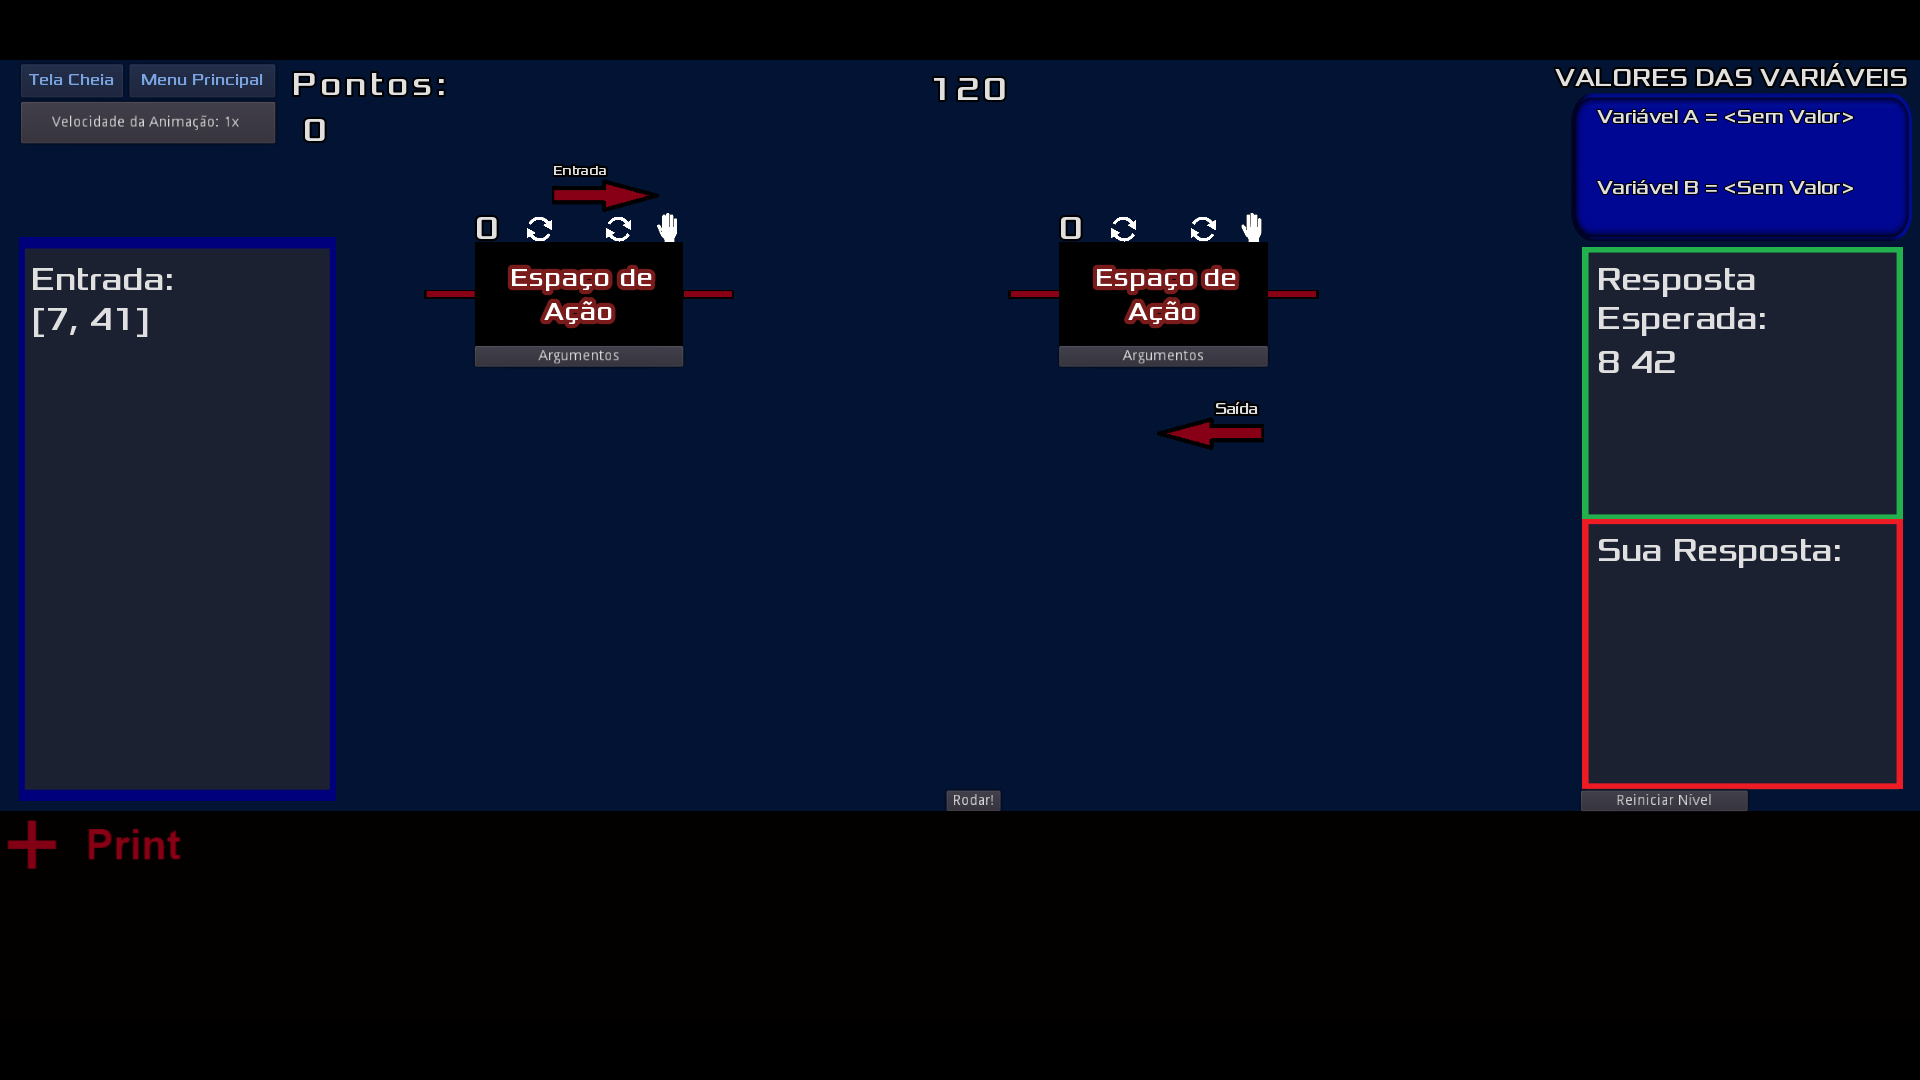
\includegraphics[width=\textwidth]{../figuras/exemplo_nivel.png}
    \caption{Exemplo de um nível}
\end{figure}

O jogador irá receber dados que serão mostrados dentro do retângulo azul, 
posicionado no lado esquerdo da tela. O exemplo abaixo mostra um nível que
fornece  ao jogador os números 7 e 41 como dados iniciais.

\begin{figure}[H]
    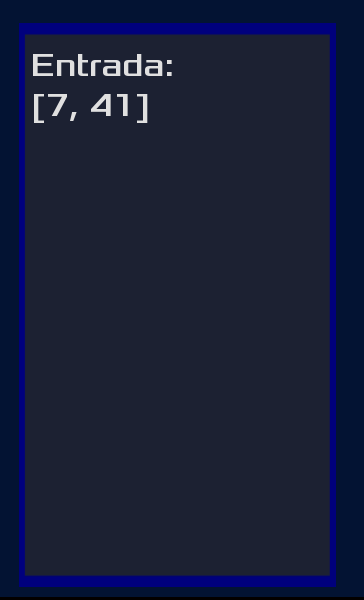
\includegraphics[scale=0.3]{../figuras/entrada.png}
    \caption{Exemplo de entrada}
\end{figure}

O objetivo do jogador é conseguir reproduzir o que está no retângulo verde, 
posicionado no lado direito da tela,
chamado "Resposta Esperada". No exemplo abaixo o nível exige que o jogador
reproduza os números 8 e 42. Após o programa do jogador ser executado a saída 
que ele obteve aparecerá abaixo de "Sua Resposta" \ que está no retângulo vermelho
(fig(a)) e caso o resultado em "Sua Resposta" \ for igual ao que está em 
"Resposta Esperada" o retângulo também ficará verde (fig (b)).

\begin{figure}[H]
    \centering
    \begin{minipage}{.4\textwidth}
      \centering
      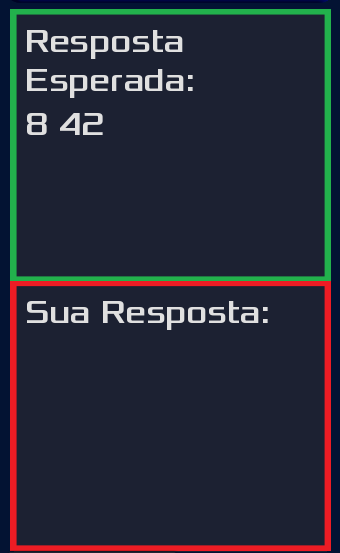
\includegraphics[scale=0.3]{../figuras/saida.png}
      \subcaption{Objetivo não alcançado}
    \end{minipage}%
    \begin{minipage}{.4\textwidth}
      \centering
      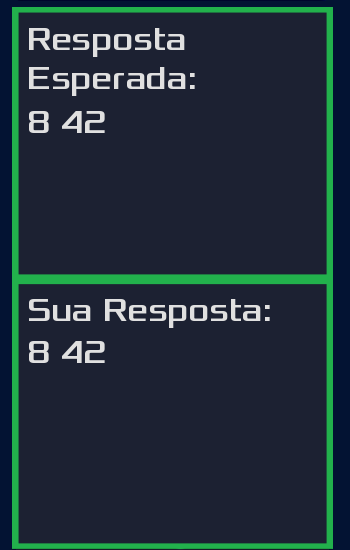
\includegraphics[scale=0.3]{../figuras/objetivo_alcancado.png}
      \subcaption{Objetivo alcançado}
    \end{minipage}
    \caption{Objetivos}
\end{figure}

O jogador deve cumprir o objetivo dentro do tempo limite para acumular pontos.
Este tempo é mostrado constantemente na tela e sempre iniciará com 120 segundos
restantes.

\begin{figure}[H]
    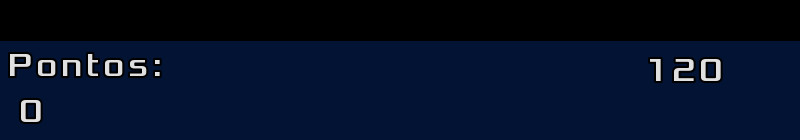
\includegraphics[scale=0.3]{../figuras/tempo_restante.png}
    \caption{Tempo restante no início do nível}
\end{figure}

Ao concluir o nível o jogador ganhará pontos iguais ao valor de tempo que 
restava ao apertar o botão "rodar!", obviamente os pontos só serão obtidos caso
o objetivo seja alcançado. Este fato está relacionado com a duração do processo 
visual que o jogo possui e será explicado mais adiante, por hora deve-se 
entender que existe um sistema de pontuação.

\begin{figure}[H]
    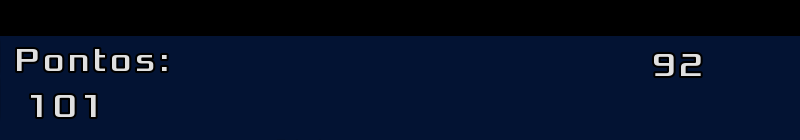
\includegraphics[scale=0.3]{../figuras/pontuacao.png}
    \caption{Pontuação obtida}
\end{figure}

Note que, se o jogador tinha zero pontos quando concluiu este nível, o programa
criado que alcançou o objetivo foi executado quando ainda havia 101 segundos
restantes, porém a animação continuou executando, consequentemente o tempo
continuou correndo, para que o usuário
pudesse visualizar o que está acontecendo durante a execução do programa criado
e aprender como funciona cada comando.

Portanto o objetivo final de \textit{Phoenix Rising} é completar o maior número
de níveis no menor tempo possível para maximizar o somatório de pontos. Para 
isso o jogador deve aprender a mecânica de jogo, o que  e como cada comando
executa sua instrução e como montar o quebra cabeça dos diferentes níveis.

\section{Elementos do Jogo}
\label{sec:consideracoes_preliminares}

Agora que o objetivo do jogo foi explicitado, deve-se entender quais elementos 
estão envolvidos para que o jogador possa concluir o desafio.

\subsection{Entrada e Saída}

Estes termos são recorrentes na computação e geralmente são chamados de
\textit{Intput} e \textit{Output} respectivamente. Neste jogo a entrada e saída
estão delimitadas pelos retângulos coloridos e servem para mostrar para o 
jogador o que ele receberá para processar e o que ele deve produzir com o código
gerado.

\begin{figure}[H]
    \centering
    \begin{minipage}{.4\textwidth}
      \centering
      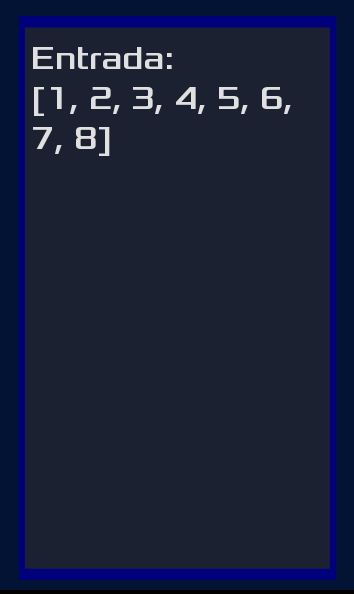
\includegraphics[scale=0.3]{../figuras/exemplo_entrada.png}
      \subcaption{Exemplo de Entrada}
    \end{minipage}%
    \begin{minipage}{.4\textwidth}
      \centering
      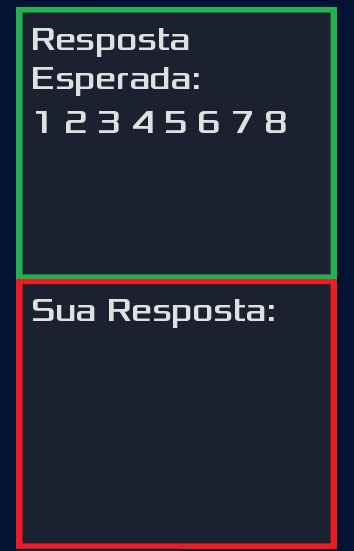
\includegraphics[scale=0.3]{../figuras/exemplo_saida.png}
      \subcaption{Exemplo de Saída}
    \end{minipage}
    \caption{Entrada e Saída}
\end{figure}

\subsection{Espaço de Ação}

Os espaços de ação são as áreas móveis do jogo que permitem montar o 
quebra-cabeças e que recebem os comandos que executarão as ações de 
processamento dos dados de entrada. Portanto este é um dos principais itens do 
jogo.

\begin{figure}[H]
    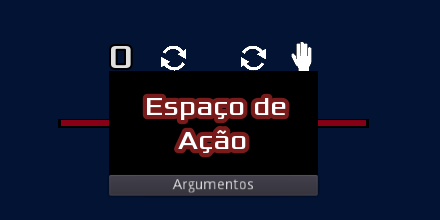
\includegraphics[width=\textwidth]{../figuras/espaco_acao.png}
    \caption{Um espaço de ação}
\end{figure}



\section{Forma de Jogar}
\label{sec:consideracoes_preliminares}

Para conseguir completar o objetivo o jogo \textit{Phoenix Rising} funciona
da seguinte forma:

O jogador deve resolver o quebra cabeças conectando os blocos da forma correta
até que a Entrada esteja conectada com a Saída.

\begin{figure}[H]
    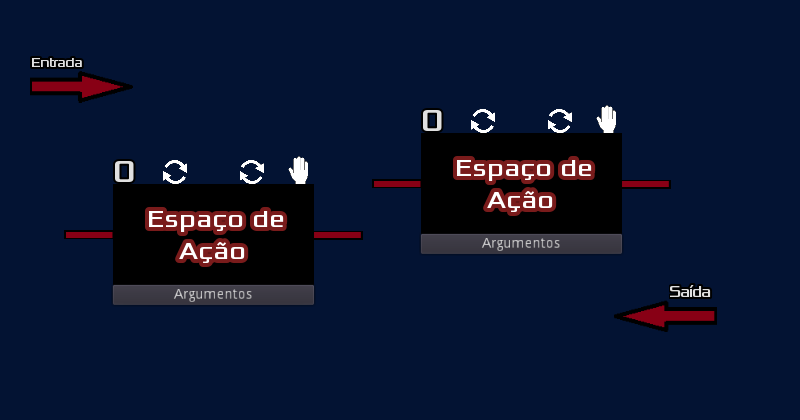
\includegraphics[width=\textwidth]{../figuras/jogo_nao_conectado.png}
    \caption{Jogo não conectado}
\end{figure}

\begin{figure}[H]
    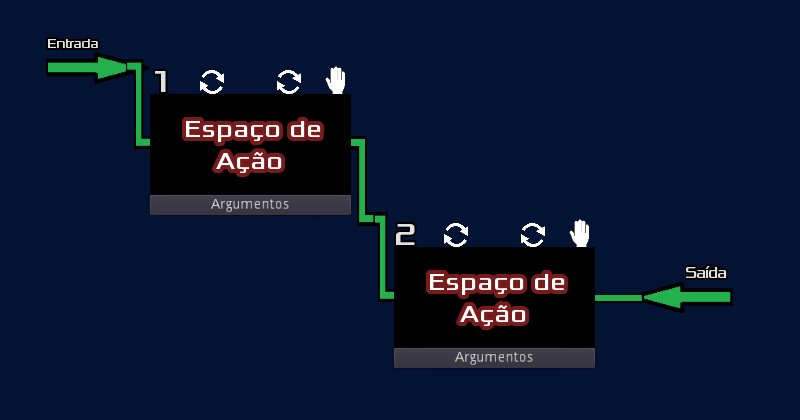
\includegraphics[width=\textwidth]{../figuras/jogo_conectado.png}
    \caption{Jogo conectado}
\end{figure}

Desta forma o jogador deve compreender que, para criar um programa, é necessário
pensar sobre a estrutura que o código terá antes de começar a utilizar os 
comandos, pois tentar criar um código apenas inserindo comandos sem pensar
previamente em uma estrutura base leva a códigos confusos e que muitas vezes
não funcionam corretamente. É claro que para sistemas maiores as reestruturações
do modelo ocorrem com certa frequência, porém o objetivo deste jogo é apenas
introduzir os conceitos básicos de programação.

Após ter o sistema conectado, o jogador deve utilizar os comandos que são
disponibilizados no inventário, posicionados no canto inferior esquerdo da tela 
de jogo.

\begin{figure}[H]
    
\includegraphics[scale=0.8]{../figuras/exemplo_comandos.png}
    \caption{Exemplo de comandos disponíveis}
\end{figure}

Depois de posicionar os comandos, o jogador deve preencher os argumentos que 
cada comando recebe e então o sistema estará pronto para ser executado.

\begin{figure}[H]
    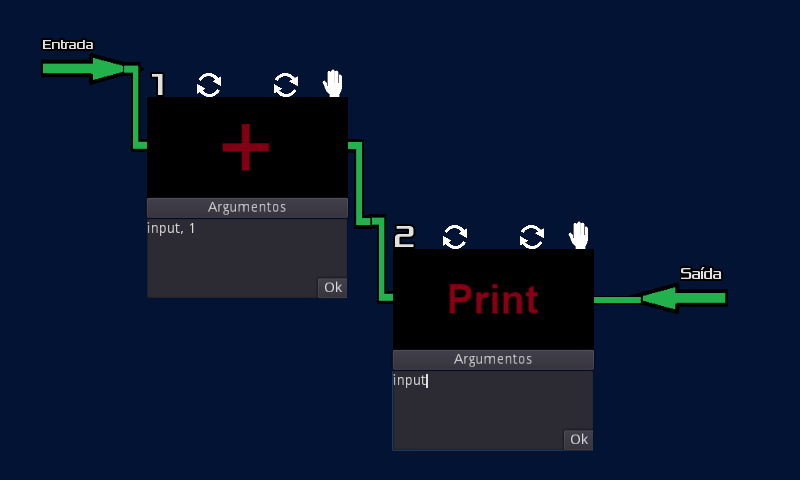
\includegraphics[width=\textwidth]{../figuras/preenchendo_argumentos.png}
    \caption{Jogador preenchendo os argumentos}
\end{figure}

Agora o sistema está pronto para ser executado.

\begin{figure}[H]
    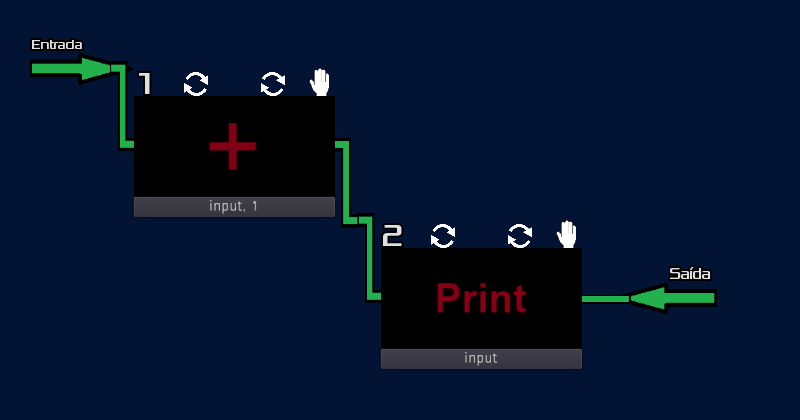
\includegraphics[width=100mm, height=80mm]{../figuras/sistema_pronto.png}
    \caption{Sistema pronto para execu\c{c}\~{a}o}
\end{figure}

Para iniciar o processamento dos dados de entrada, ou seja, rodar o programa,
basta o jogador clicar no botão \textit{rodar!} e ficar atento à animação.
No exemplo abaixo a primeira entrada era o número 7 e está sinalizada na 
animação pelo nome \textit{Input:}.

\begin{figure}[H]
    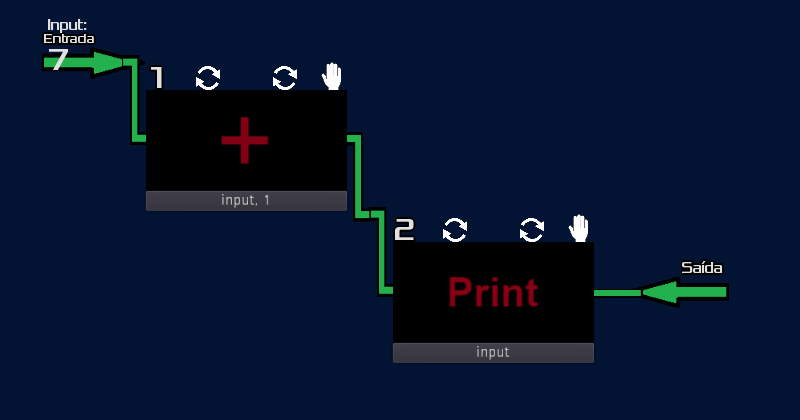
\includegraphics[width=\textwidth]{../figuras/inicio_da_execucao.png}
    \caption{Início da execu\c{c}\~{a}o do sistema}
\end{figure}

Agora o programa está rodando e o jogador pode acompanhar o que está 
acontecendo, pois o valor do \textit{Input} será exibido constantemente na tela.
Após passar por algum comando o valor de \textit{Input} será modificado de 
acordo com a operação executada.

\begin{figure}[H]
    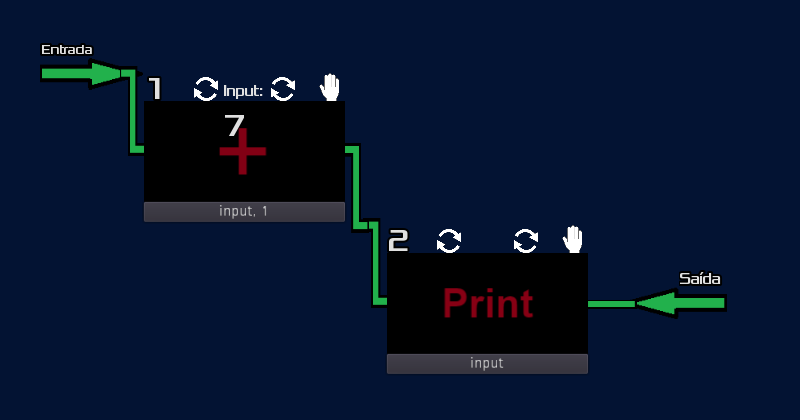
\includegraphics[width=\textwidth]{../figuras/antes_da_soma.png}
    \caption{Valor do \textit{Input} antes da opera\c{c}\~{a}o}
\end{figure}

Note que após passar pelo comando de soma, o valor de \textit{Input} será 
incrementado em 1, pois foi passado como argumento "input, 1", fazendo com que 
seja somado 1 ao valor corrente do \textit{Input}.

\begin{figure}[H]
    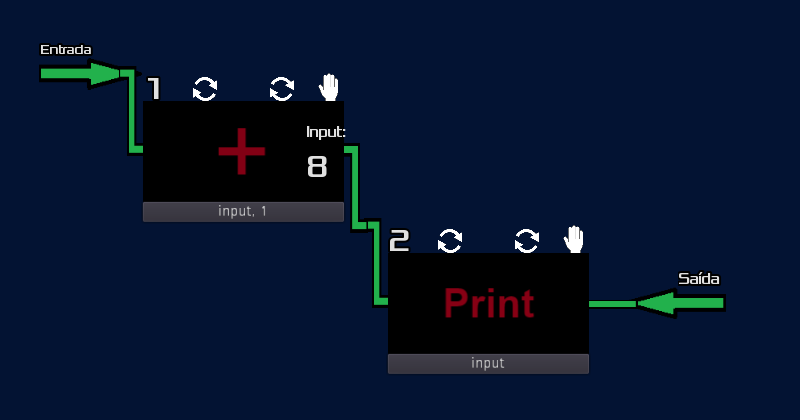
\includegraphics[width=\textwidth]{../figuras/depois_da_soma.png}
    \caption{Valor do \textit{Input} após a opera\c{c}\~{a}o}
\end{figure}

Esta maneira de conseguir acompanhar o que está acontecendo com os valores do 
programa enquanto é executada cada ação permite que o jogador entenda realmente
como cada comando funciona, facilitando o aprendizado principalmente das 
instruções que controlam o fluxo de operação e loops.

